\documentclass[1p]{elsarticle_modified}
%\bibliographystyle{elsarticle-num}

%\usepackage[colorlinks]{hyperref}
%\usepackage{abbrmath_seonhwa} %\Abb, \Ascr, \Acal ,\Abf, \Afrak
\usepackage{amsfonts}
\usepackage{amssymb}
\usepackage{amsmath}
\usepackage{amsthm}
\usepackage{scalefnt}
\usepackage{amsbsy}
\usepackage{kotex}
\usepackage{caption}
\usepackage{subfig}
\usepackage{color}
\usepackage{graphicx}
\usepackage{xcolor} %% white, black, red, green, blue, cyan, magenta, yellow
\usepackage{float}
\usepackage{setspace}
\usepackage{hyperref}

\usepackage{tikz}
\usetikzlibrary{arrows}

\usepackage{multirow}
\usepackage{array} % fixed length table
\usepackage{hhline}

%%%%%%%%%%%%%%%%%%%%%
\makeatletter
\renewcommand*\env@matrix[1][\arraystretch]{%
	\edef\arraystretch{#1}%
	\hskip -\arraycolsep
	\let\@ifnextchar\new@ifnextchar
	\array{*\c@MaxMatrixCols c}}
\makeatother %https://tex.stackexchange.com/questions/14071/how-can-i-increase-the-line-spacing-in-a-matrix
%%%%%%%%%%%%%%%

\usepackage[normalem]{ulem}

\newcommand{\msout}[1]{\ifmmode\text{\sout{\ensuremath{#1}}}\else\sout{#1}\fi}
%SOURCE: \msout is \stkout macro in https://tex.stackexchange.com/questions/20609/strikeout-in-math-mode

\newcommand{\cancel}[1]{
	\ifmmode
	{\color{red}\msout{#1}}
	\else
	{\color{red}\sout{#1}}
	\fi
}

\newcommand{\add}[1]{
	{\color{blue}\uwave{#1}}
}

\newcommand{\replace}[2]{
	\ifmmode
	{\color{red}\msout{#1}}{\color{blue}\uwave{#2}}
	\else
	{\color{red}\sout{#1}}{\color{blue}\uwave{#2}}
	\fi
}

\newcommand{\Sol}{\mathcal{S}} %segment
\newcommand{\D}{D} %diagram
\newcommand{\A}{\mathcal{A}} %arc


%%%%%%%%%%%%%%%%%%%%%%%%%%%%%5 test

\def\sl{\operatorname{\textup{SL}}(2,\Cbb)}
\def\psl{\operatorname{\textup{PSL}}(2,\Cbb)}
\def\quan{\mkern 1mu \triangleright \mkern 1mu}

\theoremstyle{definition}
\newtheorem{thm}{Theorem}[section]
\newtheorem{prop}[thm]{Proposition}
\newtheorem{lem}[thm]{Lemma}
\newtheorem{ques}[thm]{Question}
\newtheorem{cor}[thm]{Corollary}
\newtheorem{defn}[thm]{Definition}
\newtheorem{exam}[thm]{Example}
\newtheorem{rmk}[thm]{Remark}
\newtheorem{alg}[thm]{Algorithm}

\newcommand{\I}{\sqrt{-1}}
\begin{document}

%\begin{frontmatter}
%
%\title{Boundary parabolic representations of knots up to 8 crossings}
%
%%% Group authors per affiliation:
%\author{Yunhi Cho} 
%\address{Department of Mathematics, University of Seoul, Seoul, Korea}
%\ead{yhcho@uos.ac.kr}
%
%
%\author{Seonhwa Kim} %\fnref{s_kim}}
%\address{Center for Geometry and Physics, Institute for Basic Science, Pohang, 37673, Korea}
%\ead{ryeona17@ibs.re.kr}
%
%\author{Hyuk Kim}
%\address{Department of Mathematical Sciences, Seoul National University, Seoul 08826, Korea}
%\ead{hyukkim@snu.ac.kr}
%
%\author{Seokbeom Yoon}
%\address{Department of Mathematical Sciences, Seoul National University, Seoul, 08826,  Korea}
%\ead{sbyoon15@snu.ac.kr}
%
%\begin{abstract}
%We find all boundary parabolic representation of knots up to 8 crossings.
%
%\end{abstract}
%\begin{keyword}
%    \MSC[2010] 57M25 
%\end{keyword}
%
%\end{frontmatter}

%\linenumbers
%\tableofcontents
%
\newcommand\colored[1]{\textcolor{white}{\rule[-0.35ex]{0.8em}{1.4ex}}\kern-0.8em\color{red} #1}%
%\newcommand\colored[1]{\textcolor{white}{ #1}\kern-2.17ex	\textcolor{white}{ #1}\kern-1.81ex	\textcolor{white}{ #1}\kern-2.15ex\color{red}#1	}

{\Large $\underline{12n_{0849}~(K12n_{0849})}$}

\setlength{\tabcolsep}{10pt}
\renewcommand{\arraystretch}{1.6}
\vspace{1cm}\begin{tabular}{m{100pt}>{\centering\arraybackslash}m{274pt}}
\multirow{5}{120pt}{
	\centering
	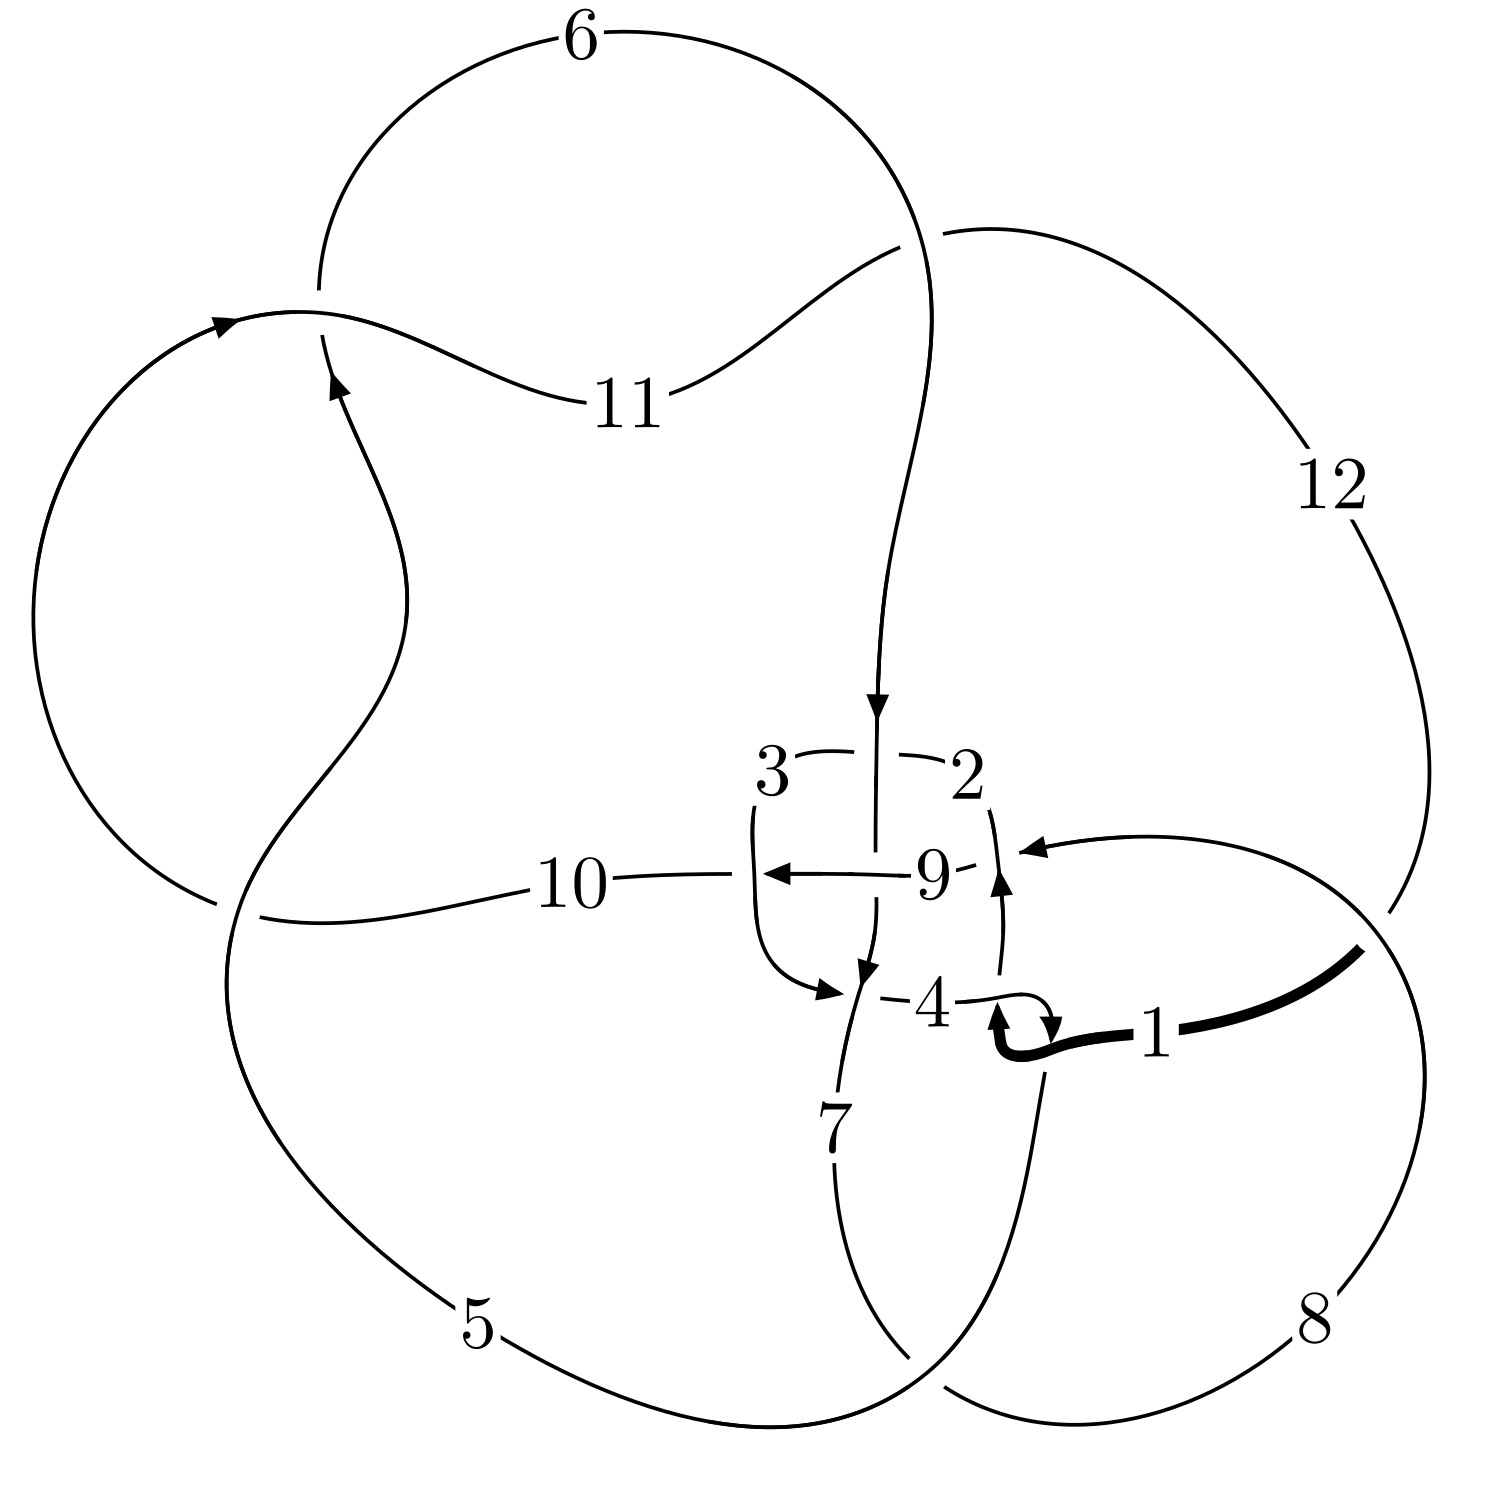
\includegraphics[width=112pt]{../../../GIT/diagram.site/Diagrams/png/2938_12n_0849.png}\\
\ \ \ A knot diagram\footnotemark}&
\allowdisplaybreaks
\textbf{Linearized knot diagam} \\
\cline{2-2}
 &
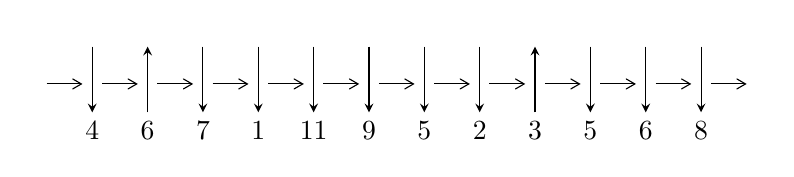
\begin{tikzpicture}[x=20pt, y=17pt]
	% nodes
	\node (C0) at (0, 0) {};
	\node (C1) at (1, 0) {};
	\node (C1U) at (1, +1) {};
	\node (C1D) at (1, -1) {4};

	\node (C2) at (2, 0) {};
	\node (C2U) at (2, +1) {};
	\node (C2D) at (2, -1) {6};

	\node (C3) at (3, 0) {};
	\node (C3U) at (3, +1) {};
	\node (C3D) at (3, -1) {7};

	\node (C4) at (4, 0) {};
	\node (C4U) at (4, +1) {};
	\node (C4D) at (4, -1) {1};

	\node (C5) at (5, 0) {};
	\node (C5U) at (5, +1) {};
	\node (C5D) at (5, -1) {11};

	\node (C6) at (6, 0) {};
	\node (C6U) at (6, +1) {};
	\node (C6D) at (6, -1) {9};

	\node (C7) at (7, 0) {};
	\node (C7U) at (7, +1) {};
	\node (C7D) at (7, -1) {5};

	\node (C8) at (8, 0) {};
	\node (C8U) at (8, +1) {};
	\node (C8D) at (8, -1) {2};

	\node (C9) at (9, 0) {};
	\node (C9U) at (9, +1) {};
	\node (C9D) at (9, -1) {3};

	\node (C10) at (10, 0) {};
	\node (C10U) at (10, +1) {};
	\node (C10D) at (10, -1) {5};

	\node (C11) at (11, 0) {};
	\node (C11U) at (11, +1) {};
	\node (C11D) at (11, -1) {6};

	\node (C12) at (12, 0) {};
	\node (C12U) at (12, +1) {};
	\node (C12D) at (12, -1) {8};
	\node (C13) at (13, 0) {};

	% arrows
	\draw[->,>={angle 60}]
	(C0) edge (C1) (C1) edge (C2) (C2) edge (C3) (C3) edge (C4) (C4) edge (C5) (C5) edge (C6) (C6) edge (C7) (C7) edge (C8) (C8) edge (C9) (C9) edge (C10) (C10) edge (C11) (C11) edge (C12) (C12) edge (C13) ;	\draw[->,>=stealth]
	(C1U) edge (C1D) (C2D) edge (C2U) (C3U) edge (C3D) (C4U) edge (C4D) (C5U) edge (C5D) (C6U) edge (C6D) (C7U) edge (C7D) (C8U) edge (C8D) (C9D) edge (C9U) (C10U) edge (C10D) (C11U) edge (C11D) (C12U) edge (C12D) ;
	\end{tikzpicture} \\
\hhline{~~} \\& 
\textbf{Solving Sequence} \\ \cline{2-2} 
 &
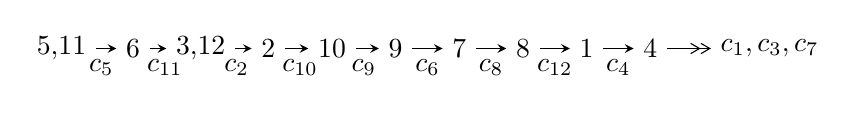
\begin{tikzpicture}[x=23pt, y=7pt]
	% node
	\node (A0) at (-1/8, 0) {5,11};
	\node (A1) at (1, 0) {6};
	\node (A2) at (33/16, 0) {3,12};
	\node (A3) at (25/8, 0) {2};
	\node (A4) at (33/8, 0) {10};
	\node (A5) at (41/8, 0) {9};
	\node (A6) at (49/8, 0) {7};
	\node (A7) at (57/8, 0) {8};
	\node (A8) at (65/8, 0) {1};
	\node (A9) at (73/8, 0) {4};
	\node (C1) at (1/2, -1) {$c_{5}$};
	\node (C2) at (3/2, -1) {$c_{11}$};
	\node (C3) at (21/8, -1) {$c_{2}$};
	\node (C4) at (29/8, -1) {$c_{10}$};
	\node (C5) at (37/8, -1) {$c_{9}$};
	\node (C6) at (45/8, -1) {$c_{6}$};
	\node (C7) at (53/8, -1) {$c_{8}$};
	\node (C8) at (61/8, -1) {$c_{12}$};
	\node (C9) at (69/8, -1) {$c_{4}$};
	\node (A10) at (11, 0) {$c_{1},c_{3},c_{7}$};

	% edge
	\draw[->,>=stealth]	
	(A0) edge (A1) (A1) edge (A2) (A2) edge (A3) (A3) edge (A4) (A4) edge (A5) (A5) edge (A6) (A6) edge (A7) (A7) edge (A8) (A8) edge (A9) ;
	\draw[->>,>={angle 60}]	
	(A9) edge (A10);
\end{tikzpicture} \\ 

\end{tabular} \\

\footnotetext{
The image of knot diagram is generated by the software ``\textbf{Draw programme}" developed by Andrew Bartholomew(\url{http://www.layer8.co.uk/maths/draw/index.htm\#Running-draw}), where we modified some parts for our purpose(\url{https://github.com/CATsTAILs/LinksPainter}).
}\phantom \\ \newline 
\centering \textbf{Ideals for irreducible components\footnotemark of $X_{\text{par}}$} 
 
\begin{align*}
I^u_{1}&=\langle 
14414381991662 u^{47}+292350624991207 u^{46}+\cdots+165519047936 b+3699504946588160,\\
\phantom{I^u_{1}}&\phantom{= \langle  }-7225595598805 u^{47}-223846226739163 u^{46}+\cdots+662076191744 a+76742753642760704,\\
\phantom{I^u_{1}}&\phantom{= \langle  }u^{48}+23 u^{47}+\cdots-16384 u-2048\rangle \\
I^u_{2}&=\langle 
-1.88889\times10^{110} a^{21} u^{2}-7.22697\times10^{109} a^{20} u^{2}+\cdots+4.85317\times10^{111} a-7.98335\times10^{111},\\
\phantom{I^u_{2}}&\phantom{= \langle  }-3 a^{21} u^2- a^{20} u^2+\cdots+95954 a+14907,\;u^3- u^2+1\rangle \\
I^u_{3}&=\langle 
-1731258 u^{33}-1052843 u^{32}+\cdots+59731 b+2238511,\\
\phantom{I^u_{3}}&\phantom{= \langle  }-2238511 u^{33}-1731258 u^{32}+\cdots+59731 a+4003959,\;u^{34}-13 u^{32}+\cdots-4 u^2+1\rangle \\
\\
\end{align*}
\raggedright * 3 irreducible components of $\dim_{\mathbb{C}}=0$, with total 148 representations.\\
\footnotetext{All coefficients of polynomials are rational numbers. But the coefficients are sometimes approximated in decimal forms when there is not enough margin.}
\newpage
\renewcommand{\arraystretch}{1}
\centering \section*{I. $I^u_{1}= \langle 1.44\times10^{13} u^{47}+2.92\times10^{14} u^{46}+\cdots+1.66\times10^{11} b+3.70\times10^{15},\;-7.23\times10^{12} u^{47}-2.24\times10^{14} u^{46}+\cdots+6.62\times10^{11} a+7.67\times10^{16},\;u^{48}+23 u^{47}+\cdots-16384 u-2048 \rangle$}
\flushleft \textbf{(i) Arc colorings}\\
\begin{tabular}{m{7pt} m{180pt} m{7pt} m{180pt} }
\flushright $a_{5}=$&$\begin{pmatrix}1\\0\end{pmatrix}$ \\
\flushright $a_{11}=$&$\begin{pmatrix}0\\u\end{pmatrix}$ \\
\flushright $a_{6}=$&$\begin{pmatrix}1\\u^2\end{pmatrix}$ \\
\flushright $a_{3}=$&$\begin{pmatrix}10.9135 u^{47}+338.097 u^{46}+\cdots-795641. u-115912.\\-87.0859 u^{47}-1766.27 u^{46}+\cdots-62895.2 u-22350.9\end{pmatrix}$ \\
\flushright $a_{12}=$&$\begin{pmatrix}- u\\- u^3+u\end{pmatrix}$ \\
\flushright $a_{2}=$&$\begin{pmatrix}-138.711 u^{47}-2931.89 u^{46}+\cdots+716421. u+84790.7\\-209.611 u^{47}-4622.85 u^{46}+\cdots+2.43872\times10^{6} u+328655.\end{pmatrix}$ \\
\flushright $a_{10}=$&$\begin{pmatrix}u\\u\end{pmatrix}$ \\
\flushright $a_{9}=$&$\begin{pmatrix}91.8720 u^{47}+2084.95 u^{46}+\cdots-1.48673\times10^{6} u-205474.\\28.1022 u^{47}+751.561 u^{46}+\cdots-1.29976\times10^{6} u-188154.\end{pmatrix}$ \\
\flushright $a_{7}=$&$\begin{pmatrix}-24.7817 u^{47}-683.674 u^{46}+\cdots+1.29959\times10^{6} u+188722.\\125.160 u^{47}+2650.22 u^{46}+\cdots-622795. u-72062.4\end{pmatrix}$ \\
\flushright $a_{8}=$&$\begin{pmatrix}-149.941 u^{47}-3333.90 u^{46}+\cdots+1.92239\times10^{6} u+260784.\\125.160 u^{47}+2650.22 u^{46}+\cdots-622795. u-72062.4\end{pmatrix}$ \\
\flushright $a_{1}=$&$\begin{pmatrix}89.8291 u^{47}+1976.87 u^{46}+\cdots-998382. u-133953.\\-50.9494 u^{47}-1049.69 u^{46}+\cdots+60359.1 u+1292.65\end{pmatrix}$ \\
\flushright $a_{4}=$&$\begin{pmatrix}113.889 u^{47}+2479.30 u^{46}+\cdots-1.06684\times10^{6} u-139256.\\51.4138 u^{47}+1243.01 u^{46}+\cdots-1.39957\times10^{6} u-199576.\end{pmatrix}$\\&\end{tabular}
\flushleft \textbf{(ii) Obstruction class $= -1$}\\~\\
\flushleft \textbf{(iii) Cusp Shapes $= \frac{16683231602363}{165519047936} u^{47}+\frac{389925962050557}{165519047936} u^{46}+\cdots-\frac{1394447538636670}{646558781} u-\frac{196913051211846}{646558781}$}\\~\\
\newpage\renewcommand{\arraystretch}{1}
\flushleft \textbf{(iv) u-Polynomials at the component}\newline \\
\begin{tabular}{m{50pt}|m{274pt}}
Crossings & \hspace{64pt}u-Polynomials at each crossing \\
\hline $$\begin{aligned}c_{1},c_{4}\end{aligned}$$&$\begin{aligned}
&u^{48}-12 u^{47}+\cdots-352 u+64
\end{aligned}$\\
\hline $$\begin{aligned}c_{2},c_{9}\end{aligned}$$&$\begin{aligned}
&u^{48}-13 u^{46}+\cdots+4 u-1
\end{aligned}$\\
\hline $$\begin{aligned}c_{3},c_{8}\end{aligned}$$&$\begin{aligned}
&u^{48}+u^{47}+\cdots+20 u-13
\end{aligned}$\\
\hline $$\begin{aligned}c_{5},c_{10},c_{11}\end{aligned}$$&$\begin{aligned}
&u^{48}-23 u^{47}+\cdots+16384 u-2048
\end{aligned}$\\
\hline $$\begin{aligned}c_{6}\end{aligned}$$&$\begin{aligned}
&u^{48}-19 u^{47}+\cdots-56 u+8
\end{aligned}$\\
\hline $$\begin{aligned}c_{7},c_{12}\end{aligned}$$&$\begin{aligned}
&u^{48}- u^{47}+\cdots+11 u-1
\end{aligned}$\\
\hline
\end{tabular}\\~\\
\newpage\renewcommand{\arraystretch}{1}
\flushleft \textbf{(v) Riley Polynomials at the component}\newline \\
\begin{tabular}{m{50pt}|m{274pt}}
Crossings & \hspace{64pt}Riley Polynomials at each crossing \\
\hline $$\begin{aligned}c_{1},c_{4}\end{aligned}$$&$\begin{aligned}
&y^{48}+26 y^{47}+\cdots-110080 y+4096
\end{aligned}$\\
\hline $$\begin{aligned}c_{2},c_{9}\end{aligned}$$&$\begin{aligned}
&y^{48}-26 y^{47}+\cdots+10 y+1
\end{aligned}$\\
\hline $$\begin{aligned}c_{3},c_{8}\end{aligned}$$&$\begin{aligned}
&y^{48}+7 y^{47}+\cdots+2616 y+169
\end{aligned}$\\
\hline $$\begin{aligned}c_{5},c_{10},c_{11}\end{aligned}$$&$\begin{aligned}
&y^{48}-27 y^{47}+\cdots-14680064 y+4194304
\end{aligned}$\\
\hline $$\begin{aligned}c_{6}\end{aligned}$$&$\begin{aligned}
&y^{48}-19 y^{47}+\cdots+1056 y+64
\end{aligned}$\\
\hline $$\begin{aligned}c_{7},c_{12}\end{aligned}$$&$\begin{aligned}
&y^{48}+33 y^{47}+\cdots-59 y+1
\end{aligned}$\\
\hline
\end{tabular}\\~\\
\newpage\flushleft \textbf{(vi) Complex Volumes and Cusp Shapes}
$$\begin{array}{c|c|c}  
\text{Solutions to }I^u_{1}& \I (\text{vol} + \sqrt{-1}CS) & \text{Cusp shape}\\
 \hline 
\begin{aligned}
u &= -0.485125 + 0.981047 I \\
a &= -1.089450 + 0.650919 I \\
b &= \phantom{-}0.110062 + 1.384580 I\end{aligned}
 & \phantom{-}8.27627 - 1.52472 I & \phantom{-0.000000 } 0 \\ \hline\begin{aligned}
u &= -0.485125 - 0.981047 I \\
a &= -1.089450 - 0.650919 I \\
b &= \phantom{-}0.110062 - 1.384580 I\end{aligned}
 & \phantom{-}8.27627 + 1.52472 I & \phantom{-0.000000 } 0 \\ \hline\begin{aligned}
u &= -0.530290 + 0.962673 I \\
a &= \phantom{-}0.901020 - 0.101260 I \\
b &= \phantom{-}0.380322 - 0.921086 I\end{aligned}
 & \phantom{-}3.99581 + 0.06032 I & \phantom{-0.000000 } 0 \\ \hline\begin{aligned}
u &= -0.530290 - 0.962673 I \\
a &= \phantom{-}0.901020 + 0.101260 I \\
b &= \phantom{-}0.380322 + 0.921086 I\end{aligned}
 & \phantom{-}3.99581 - 0.06032 I & \phantom{-0.000000 } 0 \\ \hline\begin{aligned}
u &= -0.864674 + 0.731233 I \\
a &= \phantom{-}1.25224 - 0.88853 I \\
b &= \phantom{-}0.43306 - 1.68397 I\end{aligned}
 & \phantom{-}4.75585 + 2.84058 I & \phantom{-0.000000 } 0 \\ \hline\begin{aligned}
u &= -0.864674 - 0.731233 I \\
a &= \phantom{-}1.25224 + 0.88853 I \\
b &= \phantom{-}0.43306 + 1.68397 I\end{aligned}
 & \phantom{-}4.75585 - 2.84058 I & \phantom{-0.000000 } 0 \\ \hline\begin{aligned}
u &= -0.429460 + 1.063940 I \\
a &= -0.732211 + 0.055128 I \\
b &= -0.255802 + 0.802706 I\end{aligned}
 & \phantom{-}7.68349 - 4.13518 I & \phantom{-0.000000 } 0 \\ \hline\begin{aligned}
u &= -0.429460 - 1.063940 I \\
a &= -0.732211 - 0.055128 I \\
b &= -0.255802 - 0.802706 I\end{aligned}
 & \phantom{-}7.68349 + 4.13518 I & \phantom{-0.000000 } 0 \\ \hline\begin{aligned}
u &= -0.886566 + 0.742815 I \\
a &= -1.39850 + 0.79251 I \\
b &= -0.65118 + 1.74144 I\end{aligned}
 & \phantom{-}4.69075 + 2.77591 I & \phantom{-0.000000 } 0 \\ \hline\begin{aligned}
u &= -0.886566 - 0.742815 I \\
a &= -1.39850 - 0.79251 I \\
b &= -0.65118 - 1.74144 I\end{aligned}
 & \phantom{-}4.69075 - 2.77591 I & \phantom{-0.000000 } 0\\
 \hline 
 \end{array}$$\newpage$$\begin{array}{c|c|c}  
\text{Solutions to }I^u_{1}& \I (\text{vol} + \sqrt{-1}CS) & \text{Cusp shape}\\
 \hline 
\begin{aligned}
u &= \phantom{-}1.167430 + 0.129361 I \\
a &= -0.206635 + 0.246262 I \\
b &= \phantom{-}0.273089 - 0.260763 I\end{aligned}
 & \phantom{-}1.58195 + 0.65248 I & \phantom{-0.000000 } 0 \\ \hline\begin{aligned}
u &= \phantom{-}1.167430 - 0.129361 I \\
a &= -0.206635 - 0.246262 I \\
b &= \phantom{-}0.273089 + 0.260763 I\end{aligned}
 & \phantom{-}1.58195 - 0.65248 I & \phantom{-0.000000 } 0 \\ \hline\begin{aligned}
u &= -0.494005 + 1.099620 I \\
a &= \phantom{-}0.953875 - 0.604813 I \\
b &= -0.193845 - 1.347680 I\end{aligned}
 & \phantom{-}3.09129 - 6.44202 I & \phantom{-0.000000 } 0 \\ \hline\begin{aligned}
u &= -0.494005 - 1.099620 I \\
a &= \phantom{-}0.953875 + 0.604813 I \\
b &= -0.193845 + 1.347680 I\end{aligned}
 & \phantom{-}3.09129 + 6.44202 I & \phantom{-0.000000 } 0 \\ \hline\begin{aligned}
u &= -0.552382 + 1.105430 I \\
a &= -0.909474 + 0.662368 I \\
b &= \phantom{-}0.229824 + 1.371240 I\end{aligned}
 & \phantom{-}6.60458 - 12.25780 I & \phantom{-0.000000 } 0 \\ \hline\begin{aligned}
u &= -0.552382 - 1.105430 I \\
a &= -0.909474 - 0.662368 I \\
b &= \phantom{-}0.229824 - 1.371240 I\end{aligned}
 & \phantom{-}6.60458 + 12.25780 I & \phantom{-0.000000 } 0 \\ \hline\begin{aligned}
u &= \phantom{-}0.648175 + 0.341671 I \\
a &= \phantom{-}0.150106 - 0.372567 I \\
b &= -0.224590 + 0.190202 I\end{aligned}
 & -0.314464 - 0.268937 I & -8.00000 + 0. I\phantom{ +0.000000I} \\ \hline\begin{aligned}
u &= \phantom{-}0.648175 - 0.341671 I \\
a &= \phantom{-}0.150106 + 0.372567 I \\
b &= -0.224590 - 0.190202 I\end{aligned}
 & -0.314464 + 0.268937 I & -8.00000 + 0. I\phantom{ +0.000000I} \\ \hline\begin{aligned}
u &= -0.635682 + 1.098030 I \\
a &= -0.808152 + 0.282764 I \\
b &= -0.203245 + 1.067120 I\end{aligned}
 & \phantom{-}7.01061 + 4.54766 I & \phantom{-0.000000 } 0 \\ \hline\begin{aligned}
u &= -0.635682 - 1.098030 I \\
a &= -0.808152 - 0.282764 I \\
b &= -0.203245 - 1.067120 I\end{aligned}
 & \phantom{-}7.01061 - 4.54766 I & \phantom{-0.000000 } 0\\
 \hline 
 \end{array}$$\newpage$$\begin{array}{c|c|c}  
\text{Solutions to }I^u_{1}& \I (\text{vol} + \sqrt{-1}CS) & \text{Cusp shape}\\
 \hline 
\begin{aligned}
u &= -1.278030 + 0.264389 I \\
a &= \phantom{-}0.319676 + 0.937003 I \\
b &= \phantom{-}0.656290 + 1.113000 I\end{aligned}
 & -2.93683 + 5.48157 I & \phantom{-0.000000 } 0 \\ \hline\begin{aligned}
u &= -1.278030 - 0.264389 I \\
a &= \phantom{-}0.319676 - 0.937003 I \\
b &= \phantom{-}0.656290 - 1.113000 I\end{aligned}
 & -2.93683 - 5.48157 I & \phantom{-0.000000 } 0 \\ \hline\begin{aligned}
u &= \phantom{-}0.358024 + 0.582809 I \\
a &= \phantom{-}1.062550 + 0.446046 I \\
b &= -0.120460 - 0.778961 I\end{aligned}
 & -0.94188 - 1.73288 I & -5.17947 + 1.25821 I \\ \hline\begin{aligned}
u &= \phantom{-}0.358024 - 0.582809 I \\
a &= \phantom{-}1.062550 - 0.446046 I \\
b &= -0.120460 + 0.778961 I\end{aligned}
 & -0.94188 + 1.73288 I & -5.17947 - 1.25821 I \\ \hline\begin{aligned}
u &= -1.33184\phantom{ +0.000000I} \\
a &= -0.851126\phantom{ +0.000000I} \\
b &= -1.13356\phantom{ +0.000000I}\end{aligned}
 & -6.08512\phantom{ +0.000000I} & \phantom{-0.000000 } 0 \\ \hline\begin{aligned}
u &= -1.095600 + 0.816987 I \\
a &= \phantom{-}0.865533 - 0.655040 I \\
b &= \phantom{-}0.41312 - 1.42479 I\end{aligned}
 & \phantom{-}5.53516 + 2.26996 I & \phantom{-0.000000 } 0 \\ \hline\begin{aligned}
u &= -1.095600 - 0.816987 I \\
a &= \phantom{-}0.865533 + 0.655040 I \\
b &= \phantom{-}0.41312 + 1.42479 I\end{aligned}
 & \phantom{-}5.53516 - 2.26996 I & \phantom{-0.000000 } 0 \\ \hline\begin{aligned}
u &= -1.181650 + 0.698223 I \\
a &= -0.677817 + 0.708409 I \\
b &= -0.306317 + 1.310360 I\end{aligned}
 & \phantom{-}1.93618 + 6.05436 I & \phantom{-0.000000 } 0 \\ \hline\begin{aligned}
u &= -1.181650 - 0.698223 I \\
a &= -0.677817 - 0.708409 I \\
b &= -0.306317 - 1.310360 I\end{aligned}
 & \phantom{-}1.93618 - 6.05436 I & \phantom{-0.000000 } 0 \\ \hline\begin{aligned}
u &= -1.195270 + 0.698625 I \\
a &= \phantom{-}1.37256 - 0.94570 I \\
b &= \phantom{-}0.97988 - 2.08927 I\end{aligned}
 & \phantom{-}6.06307 + 7.68979 I & \phantom{-0.000000 } 0\\
 \hline 
 \end{array}$$\newpage$$\begin{array}{c|c|c}  
\text{Solutions to }I^u_{1}& \I (\text{vol} + \sqrt{-1}CS) & \text{Cusp shape}\\
 \hline 
\begin{aligned}
u &= -1.195270 - 0.698625 I \\
a &= \phantom{-}1.37256 + 0.94570 I \\
b &= \phantom{-}0.97988 + 2.08927 I\end{aligned}
 & \phantom{-}6.06307 - 7.68979 I & \phantom{-0.000000 } 0 \\ \hline\begin{aligned}
u &= -1.18735 + 0.78240 I \\
a &= \phantom{-}1.33912 - 0.77886 I \\
b &= \phantom{-}0.98063 - 1.97251 I\end{aligned}
 & \phantom{-}4.6066 + 19.0224 I & \phantom{-0.000000 } 0 \\ \hline\begin{aligned}
u &= -1.18735 - 0.78240 I \\
a &= \phantom{-}1.33912 + 0.77886 I \\
b &= \phantom{-}0.98063 + 1.97251 I\end{aligned}
 & \phantom{-}4.6066 - 19.0224 I & \phantom{-0.000000 } 0 \\ \hline\begin{aligned}
u &= -1.20933 + 0.76456 I \\
a &= -1.30402 + 0.83062 I \\
b &= -0.94193 + 2.00149 I\end{aligned}
 & \phantom{-}0.87016 + 13.12930 I & \phantom{-0.000000 } 0 \\ \hline\begin{aligned}
u &= -1.20933 - 0.76456 I \\
a &= -1.30402 - 0.83062 I \\
b &= -0.94193 - 2.00149 I\end{aligned}
 & \phantom{-}0.87016 - 13.12930 I & \phantom{-0.000000 } 0 \\ \hline\begin{aligned}
u &= -1.23864 + 0.74371 I \\
a &= \phantom{-}0.661993 - 0.592040 I \\
b &= \phantom{-}0.379666 - 1.225650 I\end{aligned}
 & \phantom{-}5.19931 + 10.67840 I & \phantom{-0.000000 } 0 \\ \hline\begin{aligned}
u &= -1.23864 - 0.74371 I \\
a &= \phantom{-}0.661993 + 0.592040 I \\
b &= \phantom{-}0.379666 + 1.225650 I\end{aligned}
 & \phantom{-}5.19931 - 10.67840 I & \phantom{-0.000000 } 0 \\ \hline\begin{aligned}
u &= \phantom{-}0.093558 + 0.533903 I \\
a &= \phantom{-}0.324021 + 0.855715 I \\
b &= \phantom{-}0.426554 - 0.253055 I\end{aligned}
 & \phantom{-}1.21279 - 2.43642 I & -4.24996 + 4.94851 I \\ \hline\begin{aligned}
u &= \phantom{-}0.093558 - 0.533903 I \\
a &= \phantom{-}0.324021 - 0.855715 I \\
b &= \phantom{-}0.426554 + 0.253055 I\end{aligned}
 & \phantom{-}1.21279 + 2.43642 I & -4.24996 - 4.94851 I \\ \hline\begin{aligned}
u &= -1.44267 + 0.21746 I \\
a &= -0.68065 + 2.03149 I \\
b &= -0.54019 + 3.07879 I\end{aligned}
 & -6.76961 + 4.70527 I & \phantom{-0.000000 } 0\\
 \hline 
 \end{array}$$\newpage$$\begin{array}{c|c|c}  
\text{Solutions to }I^u_{1}& \I (\text{vol} + \sqrt{-1}CS) & \text{Cusp shape}\\
 \hline 
\begin{aligned}
u &= -1.44267 - 0.21746 I \\
a &= -0.68065 - 2.03149 I \\
b &= -0.54019 - 3.07879 I\end{aligned}
 & -6.76961 - 4.70527 I & \phantom{-0.000000 } 0 \\ \hline\begin{aligned}
u &= \phantom{-}1.48960 + 0.13187 I \\
a &= \phantom{-}0.305557 + 0.139429 I \\
b &= -0.436770 - 0.247989 I\end{aligned}
 & -4.21849 + 2.31870 I & \phantom{-0.000000 } 0 \\ \hline\begin{aligned}
u &= \phantom{-}1.48960 - 0.13187 I \\
a &= \phantom{-}0.305557 - 0.139429 I \\
b &= -0.436770 + 0.247989 I\end{aligned}
 & -4.21849 - 2.31870 I & \phantom{-0.000000 } 0 \\ \hline\begin{aligned}
u &= \phantom{-}1.54460 + 0.00922 I \\
a &= -0.253984 + 0.118646 I \\
b &= \phantom{-}0.393396 - 0.180918 I\end{aligned}
 & -1.53991 - 8.40513 I & \phantom{-0.000000 } 0 \\ \hline\begin{aligned}
u &= \phantom{-}1.54460 - 0.00922 I \\
a &= -0.253984 - 0.118646 I \\
b &= \phantom{-}0.393396 + 0.180918 I\end{aligned}
 & -1.53991 + 8.40513 I & \phantom{-0.000000 } 0 \\ \hline\begin{aligned}
u &= \phantom{-}0.425779\phantom{ +0.000000I} \\
a &= \phantom{-}0.565774\phantom{ +0.000000I} \\
b &= -0.240895\phantom{ +0.000000I}\end{aligned}
 & -0.780920\phantom{ +0.000000I} & -12.7940\phantom{ +0.000000I} \\ \hline\begin{aligned}
u &= -1.64161 + 0.03646 I \\
a &= -0.0546808 - 0.1253800 I \\
b &= -0.094336 - 0.203832 I\end{aligned}
 & -8.54644 + 1.50129 I & \phantom{-0.000000 } 0 \\ \hline\begin{aligned}
u &= -1.64161 - 0.03646 I \\
a &= -0.0546808 + 0.1253800 I \\
b &= -0.094336 + 0.203832 I\end{aligned}
 & -8.54644 - 1.50129 I & \phantom{-0.000000 } 0\\
 \hline 
 \end{array}$$\newpage\newpage\renewcommand{\arraystretch}{1}
\centering \section*{II. $I^u_{2}= \langle -1.89\times10^{110} a^{21} u^{2}-7.23\times10^{109} a^{20} u^{2}+\cdots+4.85\times10^{111} a-7.98\times10^{111},\;-3 a^{21} u^2- a^{20} u^2+\cdots+95954 a+14907,\;u^3- u^2+1 \rangle$}
\flushleft \textbf{(i) Arc colorings}\\
\begin{tabular}{m{7pt} m{180pt} m{7pt} m{180pt} }
\flushright $a_{5}=$&$\begin{pmatrix}1\\0\end{pmatrix}$ \\
\flushright $a_{11}=$&$\begin{pmatrix}0\\u\end{pmatrix}$ \\
\flushright $a_{6}=$&$\begin{pmatrix}1\\u^2\end{pmatrix}$ \\
\flushright $a_{3}=$&$\begin{pmatrix}a\\0.297935 a^{21} u^{2}+0.113991 a^{20} u^{2}+\cdots-7.65490 a+12.5921\end{pmatrix}$ \\
\flushright $a_{12}=$&$\begin{pmatrix}- u\\- u^2+u+1\end{pmatrix}$ \\
\flushright $a_{2}=$&$\begin{pmatrix}-0.297935 a^{21} u^{2}-0.113991 a^{20} u^{2}+\cdots+8.65490 a-12.5921\\0.105230 a^{21} u^{2}+0.223129 a^{20} u^{2}+\cdots-52.5944 a+28.7118\end{pmatrix}$ \\
\flushright $a_{10}=$&$\begin{pmatrix}u\\u\end{pmatrix}$ \\
\flushright $a_{9}=$&$\begin{pmatrix}-0.444006 a^{21} u^{2}+0.0389262 a^{20} u^{2}+\cdots-37.4768 a-1.11629\\0.219343 a^{21} u^{2}+0.183640 a^{20} u^{2}+\cdots-44.5258 a+31.9350\end{pmatrix}$ \\
\flushright $a_{7}=$&$\begin{pmatrix}-0.129004 a^{21} u^{2}+0.124229 a^{20} u^{2}+\cdots-52.7203 a+17.2976\\0.313975 a^{21} u^{2}+0.132304 a^{20} u^{2}+\cdots-3.59373 a+21.0298\end{pmatrix}$ \\
\flushright $a_{8}=$&$\begin{pmatrix}-0.442978 a^{21} u^{2}-0.00807409 a^{20} u^{2}+\cdots-49.1266 a-3.73220\\0.313975 a^{21} u^{2}+0.132304 a^{20} u^{2}+\cdots-3.59373 a+21.0298\end{pmatrix}$ \\
\flushright $a_{1}=$&$\begin{pmatrix}0.186169 a^{21} u^{2}-0.104298 a^{20} u^{2}+\cdots+39.4472 a-13.6705\\-0.314462 a^{21} u^{2}-0.0891353 a^{20} u^{2}+\cdots+5.08668 a-13.7803\end{pmatrix}$ \\
\flushright $a_{4}=$&$\begin{pmatrix}-0.180523 a^{21} u^{2}-0.0945800 a^{20} u^{2}+\cdots+2.88290 a-6.04935\\0.255393 a^{21} u^{2}+0.177825 a^{20} u^{2}+\cdots-31.5249 a+24.9875\end{pmatrix}$\\&\end{tabular}
\flushleft \textbf{(ii) Obstruction class $= -1$}\\~\\
\flushleft \textbf{(iii) Cusp Shapes $= -2.26166 a^{21} u^{2}-0.476423 a^{20} u^{2}+\cdots+4.34057 a-83.6301$}\\~\\
\newpage\renewcommand{\arraystretch}{1}
\flushleft \textbf{(iv) u-Polynomials at the component}\newline \\
\begin{tabular}{m{50pt}|m{274pt}}
Crossings & \hspace{64pt}u-Polynomials at each crossing \\
\hline $$\begin{aligned}c_{1},c_{4}\end{aligned}$$&$\begin{aligned}
&(u^{11}+3 u^{10}+\cdots+2 u+1)^{6}
\end{aligned}$\\
\hline $$\begin{aligned}c_{2},c_{9}\end{aligned}$$&$\begin{aligned}
&u^{66}-3 u^{65}+\cdots+7772 u-1789
\end{aligned}$\\
\hline $$\begin{aligned}c_{3},c_{8}\end{aligned}$$&$\begin{aligned}
&u^{66}- u^{65}+\cdots+17622 u-13807
\end{aligned}$\\
\hline $$\begin{aligned}c_{5},c_{10},c_{11}\end{aligned}$$&$\begin{aligned}
&(u^3+u^2-1)^{22}
\end{aligned}$\\
\hline $$\begin{aligned}c_{6}\end{aligned}$$&$\begin{aligned}
&(u^{11}+5 u^{10}+12 u^9+15 u^8+8 u^7-4 u^6-8 u^5-3 u^4+3 u^3+3 u^2-1)^6
\end{aligned}$\\
\hline $$\begin{aligned}c_{7},c_{12}\end{aligned}$$&$\begin{aligned}
&u^{66}+u^{65}+\cdots+509278 u-214703
\end{aligned}$\\
\hline
\end{tabular}\\~\\
\newpage\renewcommand{\arraystretch}{1}
\flushleft \textbf{(v) Riley Polynomials at the component}\newline \\
\begin{tabular}{m{50pt}|m{274pt}}
Crossings & \hspace{64pt}Riley Polynomials at each crossing \\
\hline $$\begin{aligned}c_{1},c_{4}\end{aligned}$$&$\begin{aligned}
&(y^{11}+7 y^{10}+\cdots-6 y-1)^{6}
\end{aligned}$\\
\hline $$\begin{aligned}c_{2},c_{9}\end{aligned}$$&$\begin{aligned}
&y^{66}+15 y^{65}+\cdots-174341816 y+3200521
\end{aligned}$\\
\hline $$\begin{aligned}c_{3},c_{8}\end{aligned}$$&$\begin{aligned}
&y^{66}+3 y^{65}+\cdots-190413984 y+190633249
\end{aligned}$\\
\hline $$\begin{aligned}c_{5},c_{10},c_{11}\end{aligned}$$&$\begin{aligned}
&(y^3- y^2+2 y-1)^{22}
\end{aligned}$\\
\hline $$\begin{aligned}c_{6}\end{aligned}$$&$\begin{aligned}
&(y^{11}- y^{10}+\cdots+6 y-1)^{6}
\end{aligned}$\\
\hline $$\begin{aligned}c_{7},c_{12}\end{aligned}$$&$\begin{aligned}
&y^{66}-9 y^{65}+\cdots-545194749936 y+46097378209
\end{aligned}$\\
\hline
\end{tabular}\\~\\
\newpage\flushleft \textbf{(vi) Complex Volumes and Cusp Shapes}
$$\begin{array}{c|c|c}  
\text{Solutions to }I^u_{2}& \I (\text{vol} + \sqrt{-1}CS) & \text{Cusp shape}\\
 \hline 
\begin{aligned}
u &= \phantom{-}0.877439 + 0.744862 I \\
a &= \phantom{-}0.902102 - 0.486271 I \\
b &= \phantom{-}0.320024 - 1.143140 I\end{aligned}
 & -0.99957 - 2.82812 I & -20.7516 + 2.9794 I \\ \hline\begin{aligned}
u &= \phantom{-}0.877439 + 0.744862 I \\
a &= \phantom{-}0.430794 + 0.937113 I \\
b &= -1.153740 - 0.245268 I\end{aligned}
 & -0.99957 - 2.82812 I & -20.7516 + 2.9794 I \\ \hline\begin{aligned}
u &= \phantom{-}0.877439 + 0.744862 I \\
a &= -0.552422 - 0.887606 I \\
b &= -0.098598 - 1.033000 I\end{aligned}
 & \phantom{-}0.576298 - 0.123714 I & -11.95786 + 3.06277 I \\ \hline\begin{aligned}
u &= \phantom{-}0.877439 + 0.744862 I \\
a &= -0.463244 + 0.951207 I \\
b &= -0.19763 + 1.72019 I\end{aligned}
 & \phantom{-}3.13943 - 8.75255 I & -11.6607 + 13.0030 I \\ \hline\begin{aligned}
u &= \phantom{-}0.877439 + 0.744862 I \\
a &= \phantom{-}0.646143 + 0.628778 I \\
b &= -0.176427 + 1.190300 I\end{aligned}
 & \phantom{-}0.576298 - 0.123714 I & -11.95786 + 3.06277 I \\ \hline\begin{aligned}
u &= \phantom{-}0.877439 + 0.744862 I \\
a &= \phantom{-}0.543271 + 0.997448 I \\
b &= -0.247363 + 0.953185 I\end{aligned}
 & \phantom{-}1.51685 + 2.38817 I & -8.92628 - 6.03333 I \\ \hline\begin{aligned}
u &= \phantom{-}0.877439 + 0.744862 I \\
a &= -0.372113 - 0.770438 I \\
b &= \phantom{-}0.266274 - 1.279860 I\end{aligned}
 & \phantom{-}1.51685 + 2.38817 I & -8.92628 - 6.03333 I \\ \hline\begin{aligned}
u &= \phantom{-}0.877439 + 0.744862 I \\
a &= \phantom{-}0.332427 + 1.215800 I \\
b &= \phantom{-}0.01738 + 1.77304 I\end{aligned}
 & \phantom{-}6.00992 + 2.17262 I & -0.64965 - 3.24807 I \\ \hline\begin{aligned}
u &= \phantom{-}0.877439 + 0.744862 I \\
a &= \phantom{-}1.129210 + 0.564488 I \\
b &= -0.03139 + 1.49377 I\end{aligned}
 & \phantom{-}0.955193 - 0.580337 I & -12.12606 - 2.08415 I \\ \hline\begin{aligned}
u &= \phantom{-}0.877439 + 0.744862 I \\
a &= -0.819129 - 1.007060 I \\
b &= -0.57034 - 1.33641 I\end{aligned}
 & \phantom{-}0.955193 - 0.580337 I & -12.12606 - 2.08415 I\\
 \hline 
 \end{array}$$\newpage$$\begin{array}{c|c|c}  
\text{Solutions to }I^u_{2}& \I (\text{vol} + \sqrt{-1}CS) & \text{Cusp shape}\\
 \hline 
\begin{aligned}
u &= \phantom{-}0.877439 + 0.744862 I \\
a &= \phantom{-}1.333130 - 0.022190 I \\
b &= \phantom{-}1.29442 + 1.74631 I\end{aligned}
 & \phantom{-}6.00992 - 7.82886 I & -0.64965 + 9.20696 I \\ \hline\begin{aligned}
u &= \phantom{-}0.877439 + 0.744862 I \\
a &= -1.370440 - 0.181563 I \\
b &= -1.36448 - 1.31693 I\end{aligned}
 & \phantom{-}1.51685 - 8.04441 I & -8.9263 + 11.9922 I \\ \hline\begin{aligned}
u &= \phantom{-}0.877439 + 0.744862 I \\
a &= \phantom{-}1.40246 + 0.31556 I \\
b &= \phantom{-}1.26362 + 1.15269 I\end{aligned}
 & \phantom{-}0.57630 - 5.53253 I & -11.95786 + 2.89612 I \\ \hline\begin{aligned}
u &= \phantom{-}0.877439 + 0.744862 I \\
a &= -1.43975 - 0.11169 I \\
b &= -0.75840 - 1.62760 I\end{aligned}
 & \phantom{-}0.95519 - 5.07591 I & -12.1261 + 8.0430 I \\ \hline\begin{aligned}
u &= \phantom{-}0.877439 + 0.744862 I \\
a &= -1.45028 - 0.09496 I \\
b &= -0.546673 + 0.224501 I\end{aligned}
 & \phantom{-}3.13943 + 3.09630 I & -11.66070 - 7.04410 I \\ \hline\begin{aligned}
u &= \phantom{-}0.877439 + 0.744862 I \\
a &= -1.48510 - 0.05299 I \\
b &= -0.99552 - 1.32153 I\end{aligned}
 & \phantom{-}0.57630 - 5.53253 I & -11.95786 + 2.89612 I \\ \hline\begin{aligned}
u &= \phantom{-}0.877439 + 0.744862 I \\
a &= \phantom{-}0.235861 - 0.456083 I \\
b &= \phantom{-}1.20180 + 1.16358 I\end{aligned}
 & \phantom{-}3.13943 + 3.09630 I & -11.66070 - 7.04410 I \\ \hline\begin{aligned}
u &= \phantom{-}0.877439 + 0.744862 I \\
a &= -0.83632 - 1.25050 I \\
b &= \phantom{-}1.114990 - 0.489573 I\end{aligned}
 & \phantom{-}3.13943 - 8.75255 I & -11.6607 + 13.0030 I \\ \hline\begin{aligned}
u &= \phantom{-}0.877439 + 0.744862 I \\
a &= -1.00846 - 1.16462 I \\
b &= \phantom{-}0.61392 - 1.31441 I\end{aligned}
 & \phantom{-}6.00992 + 2.17262 I & -0.64965 - 3.24807 I \\ \hline\begin{aligned}
u &= \phantom{-}0.877439 + 0.744862 I \\
a &= \phantom{-}1.41750 + 0.65162 I \\
b &= \phantom{-}1.18010 + 1.17042 I\end{aligned}
 & \phantom{-}0.95519 - 5.07591 I & -12.1261 + 8.0430 I\\
 \hline 
 \end{array}$$\newpage$$\begin{array}{c|c|c}  
\text{Solutions to }I^u_{2}& \I (\text{vol} + \sqrt{-1}CS) & \text{Cusp shape}\\
 \hline 
\begin{aligned}
u &= \phantom{-}0.877439 + 0.744862 I \\
a &= \phantom{-}1.64426 + 0.10506 I \\
b &= \phantom{-}1.06724 + 1.18010 I\end{aligned}
 & \phantom{-}1.51685 - 8.04441 I & -8.9263 + 11.9922 I \\ \hline\begin{aligned}
u &= \phantom{-}0.877439 + 0.744862 I \\
a &= -1.83928 - 0.42886 I \\
b &= -1.18627 - 0.97353 I\end{aligned}
 & \phantom{-}6.00992 - 7.82886 I & -0.64965 + 9.20696 I \\ \hline\begin{aligned}
u &= \phantom{-}0.877439 - 0.744862 I \\
a &= \phantom{-}0.902102 + 0.486271 I \\
b &= \phantom{-}0.320024 + 1.143140 I\end{aligned}
 & -0.99957 + 2.82812 I & -20.7516 - 2.9794 I \\ \hline\begin{aligned}
u &= \phantom{-}0.877439 - 0.744862 I \\
a &= \phantom{-}0.430794 - 0.937113 I \\
b &= -1.153740 + 0.245268 I\end{aligned}
 & -0.99957 + 2.82812 I & -20.7516 - 2.9794 I \\ \hline\begin{aligned}
u &= \phantom{-}0.877439 - 0.744862 I \\
a &= -0.552422 + 0.887606 I \\
b &= -0.098598 + 1.033000 I\end{aligned}
 & \phantom{-}0.576298 + 0.123714 I & -11.95786 - 3.06277 I \\ \hline\begin{aligned}
u &= \phantom{-}0.877439 - 0.744862 I \\
a &= -0.463244 - 0.951207 I \\
b &= -0.19763 - 1.72019 I\end{aligned}
 & \phantom{-}3.13943 + 8.75255 I & -11.6607 - 13.0030 I \\ \hline\begin{aligned}
u &= \phantom{-}0.877439 - 0.744862 I \\
a &= \phantom{-}0.646143 - 0.628778 I \\
b &= -0.176427 - 1.190300 I\end{aligned}
 & \phantom{-}0.576298 + 0.123714 I & -11.95786 - 3.06277 I \\ \hline\begin{aligned}
u &= \phantom{-}0.877439 - 0.744862 I \\
a &= \phantom{-}0.543271 - 0.997448 I \\
b &= -0.247363 - 0.953185 I\end{aligned}
 & \phantom{-}1.51685 - 2.38817 I & -8.92628 + 6.03333 I \\ \hline\begin{aligned}
u &= \phantom{-}0.877439 - 0.744862 I \\
a &= -0.372113 + 0.770438 I \\
b &= \phantom{-}0.266274 + 1.279860 I\end{aligned}
 & \phantom{-}1.51685 - 2.38817 I & -8.92628 + 6.03333 I \\ \hline\begin{aligned}
u &= \phantom{-}0.877439 - 0.744862 I \\
a &= \phantom{-}0.332427 - 1.215800 I \\
b &= \phantom{-}0.01738 - 1.77304 I\end{aligned}
 & \phantom{-}6.00992 - 2.17262 I & -0.64965 + 3.24807 I\\
 \hline 
 \end{array}$$\newpage$$\begin{array}{c|c|c}  
\text{Solutions to }I^u_{2}& \I (\text{vol} + \sqrt{-1}CS) & \text{Cusp shape}\\
 \hline 
\begin{aligned}
u &= \phantom{-}0.877439 - 0.744862 I \\
a &= \phantom{-}1.129210 - 0.564488 I \\
b &= -0.03139 - 1.49377 I\end{aligned}
 & \phantom{-}0.955193 + 0.580337 I & -12.12606 + 2.08415 I \\ \hline\begin{aligned}
u &= \phantom{-}0.877439 - 0.744862 I \\
a &= -0.819129 + 1.007060 I \\
b &= -0.57034 + 1.33641 I\end{aligned}
 & \phantom{-}0.955193 + 0.580337 I & -12.12606 + 2.08415 I \\ \hline\begin{aligned}
u &= \phantom{-}0.877439 - 0.744862 I \\
a &= \phantom{-}1.333130 + 0.022190 I \\
b &= \phantom{-}1.29442 - 1.74631 I\end{aligned}
 & \phantom{-}6.00992 + 7.82886 I & -0.64965 - 9.20696 I \\ \hline\begin{aligned}
u &= \phantom{-}0.877439 - 0.744862 I \\
a &= -1.370440 + 0.181563 I \\
b &= -1.36448 + 1.31693 I\end{aligned}
 & \phantom{-}1.51685 + 8.04441 I & -8.9263 - 11.9922 I \\ \hline\begin{aligned}
u &= \phantom{-}0.877439 - 0.744862 I \\
a &= \phantom{-}1.40246 - 0.31556 I \\
b &= \phantom{-}1.26362 - 1.15269 I\end{aligned}
 & \phantom{-}0.57630 + 5.53253 I & -11.95786 - 2.89612 I \\ \hline\begin{aligned}
u &= \phantom{-}0.877439 - 0.744862 I \\
a &= -1.43975 + 0.11169 I \\
b &= -0.75840 + 1.62760 I\end{aligned}
 & \phantom{-}0.95519 + 5.07591 I & -12.1261 - 8.0430 I \\ \hline\begin{aligned}
u &= \phantom{-}0.877439 - 0.744862 I \\
a &= -1.45028 + 0.09496 I \\
b &= -0.546673 - 0.224501 I\end{aligned}
 & \phantom{-}3.13943 - 3.09630 I & -11.66070 + 7.04410 I \\ \hline\begin{aligned}
u &= \phantom{-}0.877439 - 0.744862 I \\
a &= -1.48510 + 0.05299 I \\
b &= -0.99552 + 1.32153 I\end{aligned}
 & \phantom{-}0.57630 + 5.53253 I & -11.95786 - 2.89612 I \\ \hline\begin{aligned}
u &= \phantom{-}0.877439 - 0.744862 I \\
a &= \phantom{-}0.235861 + 0.456083 I \\
b &= \phantom{-}1.20180 - 1.16358 I\end{aligned}
 & \phantom{-}3.13943 - 3.09630 I & -11.66070 + 7.04410 I \\ \hline\begin{aligned}
u &= \phantom{-}0.877439 - 0.744862 I \\
a &= -0.83632 + 1.25050 I \\
b &= \phantom{-}1.114990 + 0.489573 I\end{aligned}
 & \phantom{-}3.13943 + 8.75255 I & -11.6607 - 13.0030 I\\
 \hline 
 \end{array}$$\newpage$$\begin{array}{c|c|c}  
\text{Solutions to }I^u_{2}& \I (\text{vol} + \sqrt{-1}CS) & \text{Cusp shape}\\
 \hline 
\begin{aligned}
u &= \phantom{-}0.877439 - 0.744862 I \\
a &= -1.00846 + 1.16462 I \\
b &= \phantom{-}0.61392 + 1.31441 I\end{aligned}
 & \phantom{-}6.00992 - 2.17262 I & -0.64965 + 3.24807 I \\ \hline\begin{aligned}
u &= \phantom{-}0.877439 - 0.744862 I \\
a &= \phantom{-}1.41750 - 0.65162 I \\
b &= \phantom{-}1.18010 - 1.17042 I\end{aligned}
 & \phantom{-}0.95519 + 5.07591 I & -12.1261 - 8.0430 I \\ \hline\begin{aligned}
u &= \phantom{-}0.877439 - 0.744862 I \\
a &= \phantom{-}1.64426 - 0.10506 I \\
b &= \phantom{-}1.06724 - 1.18010 I\end{aligned}
 & \phantom{-}1.51685 + 8.04441 I & -8.9263 - 11.9922 I \\ \hline\begin{aligned}
u &= \phantom{-}0.877439 - 0.744862 I \\
a &= -1.83928 + 0.42886 I \\
b &= -1.18627 + 0.97353 I\end{aligned}
 & \phantom{-}6.00992 + 7.82886 I & -0.64965 - 9.20696 I \\ \hline\begin{aligned}
u &= -0.754878\phantom{ +0.000000I} \\
a &= -0.533542 + 0.548275 I \\
b &= -0.21703 + 1.70176 I\end{aligned}
 & -3.18239 + 2.24779 I & -18.6553 - 5.0636 I \\ \hline\begin{aligned}
u &= -0.754878\phantom{ +0.000000I} \\
a &= -0.533542 - 0.548275 I \\
b &= -0.21703 - 1.70176 I\end{aligned}
 & -3.18239 - 2.24779 I & -18.6553 + 5.0636 I \\ \hline\begin{aligned}
u &= -0.754878\phantom{ +0.000000I} \\
a &= -0.279438 + 0.521422 I \\
b &= -0.747235 - 1.047170 I\end{aligned}
 & -2.62073 + 5.21629 I & -15.4555 - 9.0128 I \\ \hline\begin{aligned}
u &= -0.754878\phantom{ +0.000000I} \\
a &= -0.279438 - 0.521422 I \\
b &= -0.747235 + 1.047170 I\end{aligned}
 & -2.62073 - 5.21629 I & -15.4555 + 9.0128 I \\ \hline\begin{aligned}
u &= -0.754878\phantom{ +0.000000I} \\
a &= -0.275349 + 0.202814 I \\
b &= \phantom{-}0.183994 - 1.275850 I\end{aligned}
 & -3.56129 - 2.70441 I & -18.4871 - 0.0833 I \\ \hline\begin{aligned}
u &= -0.754878\phantom{ +0.000000I} \\
a &= -0.275349 - 0.202814 I \\
b &= \phantom{-}0.183994 + 1.275850 I\end{aligned}
 & -3.56129 + 2.70441 I & -18.4871 + 0.0833 I\\
 \hline 
 \end{array}$$\newpage$$\begin{array}{c|c|c}  
\text{Solutions to }I^u_{2}& \I (\text{vol} + \sqrt{-1}CS) & \text{Cusp shape}\\
 \hline 
\begin{aligned}
u &= -0.754878\phantom{ +0.000000I} \\
a &= -0.98988 + 1.38720 I \\
b &= -0.210941 - 0.393610 I\end{aligned}
 & -2.62073 - 5.21629 I & -15.4555 + 9.0128 I \\ \hline\begin{aligned}
u &= -0.754878\phantom{ +0.000000I} \\
a &= -0.98988 - 1.38720 I \\
b &= -0.210941 + 0.393610 I\end{aligned}
 & -2.62073 + 5.21629 I & -15.4555 - 9.0128 I \\ \hline\begin{aligned}
u &= -0.754878\phantom{ +0.000000I} \\
a &= \phantom{-}0.24374 + 1.69014 I \\
b &= -0.207855 - 0.153100 I\end{aligned}
 & -3.56129 + 2.70441 I & -18.4871 + 0.0833 I \\ \hline\begin{aligned}
u &= -0.754878\phantom{ +0.000000I} \\
a &= \phantom{-}0.24374 - 1.69014 I \\
b &= -0.207855 + 0.153100 I\end{aligned}
 & -3.56129 - 2.70441 I & -18.4871 - 0.0833 I \\ \hline\begin{aligned}
u &= -0.754878\phantom{ +0.000000I} \\
a &= \phantom{-}1.33232 + 1.38795 I \\
b &= \phantom{-}1.53989 + 0.03375 I\end{aligned}
 & \phantom{-}1.87234 - 5.00074 I & -7.17892 + 6.22751 I \\ \hline\begin{aligned}
u &= -0.754878\phantom{ +0.000000I} \\
a &= \phantom{-}1.33232 - 1.38795 I \\
b &= \phantom{-}1.53989 - 0.03375 I\end{aligned}
 & \phantom{-}1.87234 + 5.00074 I & -7.17892 - 6.22751 I \\ \hline\begin{aligned}
u &= -0.754878\phantom{ +0.000000I} \\
a &= \phantom{-}2.03992 + 0.04471 I \\
b &= \phantom{-}1.00574 + 1.04773 I\end{aligned}
 & \phantom{-}1.87234 - 5.00074 I & -7.17892 + 6.22751 I \\ \hline\begin{aligned}
u &= -0.754878\phantom{ +0.000000I} \\
a &= \phantom{-}2.03992 - 0.04471 I \\
b &= \phantom{-}1.00574 - 1.04773 I\end{aligned}
 & \phantom{-}1.87234 + 5.00074 I & -7.17892 - 6.22751 I \\ \hline\begin{aligned}
u &= -0.754878\phantom{ +0.000000I} \\
a &= -0.28750 + 2.25436 I \\
b &= -0.402759 + 0.413881 I\end{aligned}
 & -3.18239 + 2.24779 I & -18.6553 - 5.0636 I \\ \hline\begin{aligned}
u &= -0.754878\phantom{ +0.000000I} \\
a &= -0.28750 - 2.25436 I \\
b &= -0.402759 - 0.413881 I\end{aligned}
 & -3.18239 - 2.24779 I & -18.6553 + 5.0636 I\\
 \hline 
 \end{array}$$\newpage$$\begin{array}{c|c|c}  
\text{Solutions to }I^u_{2}& \I (\text{vol} + \sqrt{-1}CS) & \text{Cusp shape}\\
 \hline 
\begin{aligned}
u &= -0.754878\phantom{ +0.000000I} \\
a &= \phantom{-}2.95304 + 0.44701 I \\
b &= \phantom{-}3.18424 + 0.20464 I\end{aligned}
 & -0.99816 + 5.92443 I & \phantom{-0.000000 } 0 \\ \hline\begin{aligned}
u &= -0.754878\phantom{ +0.000000I} \\
a &= \phantom{-}2.95304 - 0.44701 I \\
b &= \phantom{-}3.18424 - 0.20464 I\end{aligned}
 & -0.99816 - 5.92443 I & \phantom{-0.000000 } 0 \\ \hline\begin{aligned}
u &= -0.754878\phantom{ +0.000000I} \\
a &= -3.15422\phantom{ +0.000000I} \\
b &= -3.35926\phantom{ +0.000000I}\end{aligned}
 & -5.13715\phantom{ +0.000000I} & \phantom{-0.000000 } 0 \\ \hline\begin{aligned}
u &= -0.754878\phantom{ +0.000000I} \\
a &= \phantom{-}4.21822 + 0.27109 I \\
b &= \phantom{-}2.22919 + 0.33744 I\end{aligned}
 & -0.99816 + 5.92443 I & \phantom{-0.000000 } 0 \\ \hline\begin{aligned}
u &= -0.754878\phantom{ +0.000000I} \\
a &= \phantom{-}4.21822 - 0.27109 I \\
b &= \phantom{-}2.22919 - 0.33744 I\end{aligned}
 & -0.99816 - 5.92443 I & \phantom{-0.000000 } 0 \\ \hline\begin{aligned}
u &= -0.754878\phantom{ +0.000000I} \\
a &= -4.45007\phantom{ +0.000000I} \\
b &= -2.38105\phantom{ +0.000000I}\end{aligned}
 & -5.13715\phantom{ +0.000000I} & \phantom{-0.000000 } 0\\
 \hline 
 \end{array}$$\newpage\newpage\renewcommand{\arraystretch}{1}
\centering \section*{III. $I^u_{3}= \langle -1.73\times10^{6} u^{33}-1.05\times10^{6} u^{32}+\cdots+5.97\times10^{4} b+2.24\times10^{6},\;-2.24\times10^{6} u^{33}-1.73\times10^{6} u^{32}+\cdots+5.97\times10^{4} a+4.00\times10^{6},\;u^{34}-13 u^{32}+\cdots-4 u^2+1 \rangle$}
\flushleft \textbf{(i) Arc colorings}\\
\begin{tabular}{m{7pt} m{180pt} m{7pt} m{180pt} }
\flushright $a_{5}=$&$\begin{pmatrix}1\\0\end{pmatrix}$ \\
\flushright $a_{11}=$&$\begin{pmatrix}0\\u\end{pmatrix}$ \\
\flushright $a_{6}=$&$\begin{pmatrix}1\\u^2\end{pmatrix}$ \\
\flushright $a_{3}=$&$\begin{pmatrix}37.4765 u^{33}+28.9842 u^{32}+\cdots-72.4005 u-67.0332\\28.9842 u^{33}+17.6264 u^{32}+\cdots-67.0332 u-37.4765\end{pmatrix}$ \\
\flushright $a_{12}=$&$\begin{pmatrix}- u\\- u^3+u\end{pmatrix}$ \\
\flushright $a_{2}=$&$\begin{pmatrix}26.1187 u^{33}+23.6640 u^{32}+\cdots-42.8439 u-58.5409\\24.4307 u^{33}+15.0188 u^{32}+\cdots-55.6753 u-32.1563\end{pmatrix}$ \\
\flushright $a_{10}=$&$\begin{pmatrix}u\\u\end{pmatrix}$ \\
\flushright $a_{9}=$&$\begin{pmatrix}10.4182 u^{33}-5.53038 u^{32}+\cdots-32.7393 u+13.5756\\-5.53038 u^{33}+2.99749 u^{32}+\cdots+14.5756 u-10.4182\end{pmatrix}$ \\
\flushright $a_{7}=$&$\begin{pmatrix}29.5853 u^{33}-19.1478 u^{32}+\cdots-80.7177 u+59.8427\\-12.3570 u^{33}+6.32862 u^{32}+\cdots+34.3663 u-16.4659\end{pmatrix}$ \\
\flushright $a_{8}=$&$\begin{pmatrix}41.9423 u^{33}-25.4764 u^{32}+\cdots-115.084 u+76.3086\\-12.3570 u^{33}+6.32862 u^{32}+\cdots+34.3663 u-16.4659\end{pmatrix}$ \\
\flushright $a_{1}=$&$\begin{pmatrix}-6.60429 u^{33}+10.0088 u^{32}+\cdots+16.9741 u-26.1847\\6.17162 u^{33}+0.380154 u^{32}+\cdots-18.5804 u-3.40451\end{pmatrix}$ \\
\flushright $a_{4}=$&$\begin{pmatrix}16.7796 u^{33}+11.6363 u^{32}+\cdots-45.8180 u-28.3939\\15.6963 u^{33}+8.48193 u^{32}+\cdots-36.5974 u-21.8641\end{pmatrix}$\\&\end{tabular}
\flushleft \textbf{(ii) Obstruction class $= 1$}\\~\\
\flushleft \textbf{(iii) Cusp Shapes $= -\frac{663479}{59731} u^{33}+\frac{1468982}{59731} u^{32}+\cdots+\frac{3288260}{59731} u-\frac{4500469}{59731}$}\\~\\
\newpage\renewcommand{\arraystretch}{1}
\flushleft \textbf{(iv) u-Polynomials at the component}\newline \\
\begin{tabular}{m{50pt}|m{274pt}}
Crossings & \hspace{64pt}u-Polynomials at each crossing \\
\hline $$\begin{aligned}c_{1}\end{aligned}$$&$\begin{aligned}
&u^{34}-11 u^{33}+\cdots-153 u+25
\end{aligned}$\\
\hline $$\begin{aligned}c_{2},c_{9}\end{aligned}$$&$\begin{aligned}
&u^{34}+8 u^{32}+\cdots+4 u-1
\end{aligned}$\\
\hline $$\begin{aligned}c_{3},c_{8}\end{aligned}$$&$\begin{aligned}
&u^{34}+u^{33}+\cdots+4 u-1
\end{aligned}$\\
\hline $$\begin{aligned}c_{4}\end{aligned}$$&$\begin{aligned}
&u^{34}+11 u^{33}+\cdots+153 u+25
\end{aligned}$\\
\hline $$\begin{aligned}c_{5}\end{aligned}$$&$\begin{aligned}
&u^{34}-13 u^{32}+\cdots-4 u^2+1
\end{aligned}$\\
\hline $$\begin{aligned}c_{6}\end{aligned}$$&$\begin{aligned}
&u^{34}-22 u^{33}+\cdots-11 u+1
\end{aligned}$\\
\hline $$\begin{aligned}c_{7},c_{12}\end{aligned}$$&$\begin{aligned}
&u^{34}+u^{33}+\cdots+7 u-1
\end{aligned}$\\
\hline $$\begin{aligned}c_{10},c_{11}\end{aligned}$$&$\begin{aligned}
&u^{34}-13 u^{32}+\cdots-4 u^2+1
\end{aligned}$\\
\hline
\end{tabular}\\~\\
\newpage\renewcommand{\arraystretch}{1}
\flushleft \textbf{(v) Riley Polynomials at the component}\newline \\
\begin{tabular}{m{50pt}|m{274pt}}
Crossings & \hspace{64pt}Riley Polynomials at each crossing \\
\hline $$\begin{aligned}c_{1},c_{4}\end{aligned}$$&$\begin{aligned}
&y^{34}+19 y^{33}+\cdots+9841 y+625
\end{aligned}$\\
\hline $$\begin{aligned}c_{2},c_{9}\end{aligned}$$&$\begin{aligned}
&y^{34}+16 y^{33}+\cdots+6 y+1
\end{aligned}$\\
\hline $$\begin{aligned}c_{3},c_{8}\end{aligned}$$&$\begin{aligned}
&y^{34}-3 y^{33}+\cdots+4 y+1
\end{aligned}$\\
\hline $$\begin{aligned}c_{5},c_{10},c_{11}\end{aligned}$$&$\begin{aligned}
&y^{34}-26 y^{33}+\cdots-8 y+1
\end{aligned}$\\
\hline $$\begin{aligned}c_{6}\end{aligned}$$&$\begin{aligned}
&y^{34}-18 y^{33}+\cdots-13 y+1
\end{aligned}$\\
\hline $$\begin{aligned}c_{7},c_{12}\end{aligned}$$&$\begin{aligned}
&y^{34}-17 y^{33}+\cdots-23 y+1
\end{aligned}$\\
\hline
\end{tabular}\\~\\
\newpage\flushleft \textbf{(vi) Complex Volumes and Cusp Shapes}
$$\begin{array}{c|c|c}  
\text{Solutions to }I^u_{3}& \I (\text{vol} + \sqrt{-1}CS) & \text{Cusp shape}\\
 \hline 
\begin{aligned}
u &= \phantom{-}0.845244 + 0.604160 I \\
a &= \phantom{-}1.91410 + 0.14388 I \\
b &= \phantom{-}1.53095 + 1.27804 I\end{aligned}
 & \phantom{-}3.25368 - 6.85148 I & -4.85043 + 7.91334 I \\ \hline\begin{aligned}
u &= \phantom{-}0.845244 - 0.604160 I \\
a &= \phantom{-}1.91410 - 0.14388 I \\
b &= \phantom{-}1.53095 - 1.27804 I\end{aligned}
 & \phantom{-}3.25368 + 6.85148 I & -4.85043 - 7.91334 I \\ \hline\begin{aligned}
u &= -0.895619 + 0.699368 I \\
a &= -0.590494 + 0.168532 I \\
b &= \phantom{-}0.410992 - 0.563913 I\end{aligned}
 & \phantom{-}4.00733 - 2.65022 I & -2.94134 + 1.85323 I \\ \hline\begin{aligned}
u &= -0.895619 - 0.699368 I \\
a &= -0.590494 - 0.168532 I \\
b &= \phantom{-}0.410992 + 0.563913 I\end{aligned}
 & \phantom{-}4.00733 + 2.65022 I & -2.94134 - 1.85323 I \\ \hline\begin{aligned}
u &= -0.853323 + 0.773155 I \\
a &= \phantom{-}0.589236 - 0.220815 I \\
b &= -0.332084 + 0.643997 I\end{aligned}
 & -0.36168 + 2.92655 I & -4.69868 - 5.16619 I \\ \hline\begin{aligned}
u &= -0.853323 - 0.773155 I \\
a &= \phantom{-}0.589236 + 0.220815 I \\
b &= -0.332084 - 0.643997 I\end{aligned}
 & -0.36168 - 2.92655 I & -4.69868 + 5.16619 I \\ \hline\begin{aligned}
u &= -0.898698 + 0.721304 I \\
a &= -0.471500 + 0.227103 I \\
b &= \phantom{-}0.259926 - 0.544192 I\end{aligned}
 & \phantom{-}3.97518 + 8.07880 I & -4.76528 - 6.64300 I \\ \hline\begin{aligned}
u &= -0.898698 - 0.721304 I \\
a &= -0.471500 - 0.227103 I \\
b &= \phantom{-}0.259926 + 0.544192 I\end{aligned}
 & \phantom{-}3.97518 - 8.07880 I & -4.76528 + 6.64300 I \\ \hline\begin{aligned}
u &= \phantom{-}0.857194 + 0.802437 I \\
a &= -1.350540 - 0.116108 I \\
b &= -1.06450 - 1.18325 I\end{aligned}
 & \phantom{-}1.52615 - 6.51453 I & -5.61054 + 6.02417 I \\ \hline\begin{aligned}
u &= \phantom{-}0.857194 - 0.802437 I \\
a &= -1.350540 + 0.116108 I \\
b &= -1.06450 + 1.18325 I\end{aligned}
 & \phantom{-}1.52615 + 6.51453 I & -5.61054 - 6.02417 I\\
 \hline 
 \end{array}$$\newpage$$\begin{array}{c|c|c}  
\text{Solutions to }I^u_{3}& \I (\text{vol} + \sqrt{-1}CS) & \text{Cusp shape}\\
 \hline 
\begin{aligned}
u &= -1.187710 + 0.191526 I \\
a &= -0.041458 - 0.375482 I \\
b &= \phantom{-}0.121155 + 0.438023 I\end{aligned}
 & -4.19227 + 6.40599 I & -15.5049 - 8.8278 I \\ \hline\begin{aligned}
u &= -1.187710 - 0.191526 I \\
a &= -0.041458 + 0.375482 I \\
b &= \phantom{-}0.121155 - 0.438023 I\end{aligned}
 & -4.19227 - 6.40599 I & -15.5049 + 8.8278 I \\ \hline\begin{aligned}
u &= \phantom{-}1.027460 + 0.661768 I \\
a &= -0.303568 - 0.915936 I \\
b &= \phantom{-}0.294234 - 1.141980 I\end{aligned}
 & \phantom{-}2.64248 + 1.96167 I & -1.53326 - 1.99100 I \\ \hline\begin{aligned}
u &= \phantom{-}1.027460 - 0.661768 I \\
a &= -0.303568 + 0.915936 I \\
b &= \phantom{-}0.294234 + 1.141980 I\end{aligned}
 & \phantom{-}2.64248 - 1.96167 I & -1.53326 + 1.99100 I \\ \hline\begin{aligned}
u &= \phantom{-}1.22760\phantom{ +0.000000I} \\
a &= -1.93511\phantom{ +0.000000I} \\
b &= -2.37554\phantom{ +0.000000I}\end{aligned}
 & -6.94043\phantom{ +0.000000I} & -24.4110\phantom{ +0.000000I} \\ \hline\begin{aligned}
u &= \phantom{-}0.905250 + 0.844336 I \\
a &= \phantom{-}0.550716 + 0.724589 I \\
b &= -0.113261 + 1.120920 I\end{aligned}
 & \phantom{-}1.39644 + 0.41153 I & -2.71773 - 1.79950 I \\ \hline\begin{aligned}
u &= \phantom{-}0.905250 - 0.844336 I \\
a &= \phantom{-}0.550716 - 0.724589 I \\
b &= -0.113261 - 1.120920 I\end{aligned}
 & \phantom{-}1.39644 - 0.41153 I & -2.71773 + 1.79950 I \\ \hline\begin{aligned}
u &= \phantom{-}1.232980 + 0.132443 I \\
a &= \phantom{-}1.43939 - 0.87127 I \\
b &= \phantom{-}1.89014 - 0.88362 I\end{aligned}
 & -2.81974 - 6.65969 I & -13.9389 + 9.7504 I \\ \hline\begin{aligned}
u &= \phantom{-}1.232980 - 0.132443 I \\
a &= \phantom{-}1.43939 + 0.87127 I \\
b &= \phantom{-}1.89014 + 0.88362 I\end{aligned}
 & -2.81974 + 6.65969 I & -13.9389 - 9.7504 I \\ \hline\begin{aligned}
u &= -1.249730 + 0.109070 I \\
a &= \phantom{-}0.268415 - 0.308268 I \\
b &= -0.301823 + 0.414527 I\end{aligned}
 & -5.53822 - 1.91820 I & -16.6362 + 1.6027 I\\
 \hline 
 \end{array}$$\newpage$$\begin{array}{c|c|c}  
\text{Solutions to }I^u_{3}& \I (\text{vol} + \sqrt{-1}CS) & \text{Cusp shape}\\
 \hline 
\begin{aligned}
u &= -1.249730 - 0.109070 I \\
a &= \phantom{-}0.268415 + 0.308268 I \\
b &= -0.301823 - 0.414527 I\end{aligned}
 & -5.53822 + 1.91820 I & -16.6362 - 1.6027 I \\ \hline\begin{aligned}
u &= \phantom{-}0.665736\phantom{ +0.000000I} \\
a &= -4.03140\phantom{ +0.000000I} \\
b &= -2.68384\phantom{ +0.000000I}\end{aligned}
 & -4.67762\phantom{ +0.000000I} & -5.42070\phantom{ +0.000000I} \\ \hline\begin{aligned}
u &= -0.648923 + 0.147922 I \\
a &= \phantom{-}0.761243 - 0.982468 I \\
b &= -0.348659 + 0.750150 I\end{aligned}
 & -2.03261 - 4.84635 I & -3.32627 + 1.12061 I \\ \hline\begin{aligned}
u &= -0.648923 - 0.147922 I \\
a &= \phantom{-}0.761243 + 0.982468 I \\
b &= -0.348659 - 0.750150 I\end{aligned}
 & -2.03261 + 4.84635 I & -3.32627 - 1.12061 I \\ \hline\begin{aligned}
u &= \phantom{-}0.659269 + 0.077443 I \\
a &= \phantom{-}4.04500 - 0.28467 I \\
b &= \phantom{-}2.68879 + 0.12558 I\end{aligned}
 & -0.48875 + 5.72099 I & -1.66381 - 3.21415 I \\ \hline\begin{aligned}
u &= \phantom{-}0.659269 - 0.077443 I \\
a &= \phantom{-}4.04500 + 0.28467 I \\
b &= \phantom{-}2.68879 - 0.12558 I\end{aligned}
 & -0.48875 - 5.72099 I & -1.66381 + 3.21415 I \\ \hline\begin{aligned}
u &= -0.595318 + 0.097089 I \\
a &= -0.052986 - 1.365210 I \\
b &= \phantom{-}0.164091 + 0.807592 I\end{aligned}
 & -2.91383 + 2.92551 I & -4.46735 - 4.14484 I \\ \hline\begin{aligned}
u &= -0.595318 - 0.097089 I \\
a &= -0.052986 + 1.365210 I \\
b &= \phantom{-}0.164091 - 0.807592 I\end{aligned}
 & -2.91383 - 2.92551 I & -4.46735 + 4.14484 I \\ \hline\begin{aligned}
u &= \phantom{-}1.42516 + 0.21887 I \\
a &= -0.74184 - 2.07454 I \\
b &= -0.60318 - 3.11893 I\end{aligned}
 & -6.84248 - 4.69187 I & -65.0121 + 0. I\phantom{ +0.000000I} \\ \hline\begin{aligned}
u &= \phantom{-}1.42516 - 0.21887 I \\
a &= -0.74184 + 2.07454 I \\
b &= -0.60318 + 3.11893 I\end{aligned}
 & -6.84248 + 4.69187 I & -65.0121 + 0. I\phantom{ +0.000000I}\\
 \hline 
 \end{array}$$\newpage$$\begin{array}{c|c|c}  
\text{Solutions to }I^u_{3}& \I (\text{vol} + \sqrt{-1}CS) & \text{Cusp shape}\\
 \hline 
\begin{aligned}
u &= -1.62951 + 0.02230 I \\
a &= \phantom{-}0.0272909 + 0.0596106 I \\
b &= -0.0458005 - 0.0965277 I\end{aligned}
 & -8.58478 + 1.54555 I & \phantom{-0.000000 } 0 \\ \hline\begin{aligned}
u &= -1.62951 - 0.02230 I \\
a &= \phantom{-}0.0272909 - 0.0596106 I \\
b &= -0.0458005 + 0.0965277 I\end{aligned}
 & -8.58478 - 1.54555 I & \phantom{-0.000000 } 0 \\ \hline\begin{aligned}
u &= \phantom{-}0.059608 + 0.333902 I \\
a &= \phantom{-}2.94025 + 0.58858 I \\
b &= -0.021265 + 1.016840 I\end{aligned}
 & -1.89189 + 2.22619 I & -11.47365 - 4.34728 I \\ \hline\begin{aligned}
u &= \phantom{-}0.059608 - 0.333902 I \\
a &= \phantom{-}2.94025 - 0.58858 I \\
b &= -0.021265 - 1.016840 I\end{aligned}
 & -1.89189 - 2.22619 I & -11.47365 + 4.34728 I\\
 \hline 
 \end{array}$$\newpage
\newpage\renewcommand{\arraystretch}{1}
\centering \section*{ IV. u-Polynomials}
\begin{tabular}{m{50pt}|m{274pt}}
Crossings & \hspace{64pt}u-Polynomials at each crossing \\
\hline $$\begin{aligned}c_{1}\end{aligned}$$&$\begin{aligned}
&((u^{11}+3 u^{10}+\cdots+2 u+1)^{6})(u^{34}-11 u^{33}+\cdots-153 u+25)\\
&\cdot(u^{48}-12 u^{47}+\cdots-352 u+64)
\end{aligned}$\\
\hline $$\begin{aligned}c_{2},c_{9}\end{aligned}$$&$\begin{aligned}
&(u^{34}+8 u^{32}+\cdots+4 u-1)(u^{48}-13 u^{46}+\cdots+4 u-1)\\
&\cdot(u^{66}-3 u^{65}+\cdots+7772 u-1789)
\end{aligned}$\\
\hline $$\begin{aligned}c_{3},c_{8}\end{aligned}$$&$\begin{aligned}
&(u^{34}+u^{33}+\cdots+4 u-1)(u^{48}+u^{47}+\cdots+20 u-13)\\
&\cdot(u^{66}- u^{65}+\cdots+17622 u-13807)
\end{aligned}$\\
\hline $$\begin{aligned}c_{4}\end{aligned}$$&$\begin{aligned}
&((u^{11}+3 u^{10}+\cdots+2 u+1)^{6})(u^{34}+11 u^{33}+\cdots+153 u+25)\\
&\cdot(u^{48}-12 u^{47}+\cdots-352 u+64)
\end{aligned}$\\
\hline $$\begin{aligned}c_{5}\end{aligned}$$&$\begin{aligned}
&((u^3+u^2-1)^{22})(u^{34}-13 u^{32}+\cdots-4 u^2+1)\\
&\cdot(u^{48}-23 u^{47}+\cdots+16384 u-2048)
\end{aligned}$\\
\hline $$\begin{aligned}c_{6}\end{aligned}$$&$\begin{aligned}
&(u^{11}+5 u^{10}+12 u^9+15 u^8+8 u^7-4 u^6-8 u^5-3 u^4+3 u^3+3 u^2-1)^6\\
&\cdot(u^{34}-22 u^{33}+\cdots-11 u+1)(u^{48}-19 u^{47}+\cdots-56 u+8)
\end{aligned}$\\
\hline $$\begin{aligned}c_{7},c_{12}\end{aligned}$$&$\begin{aligned}
&(u^{34}+u^{33}+\cdots+7 u-1)(u^{48}- u^{47}+\cdots+11 u-1)\\
&\cdot(u^{66}+u^{65}+\cdots+509278 u-214703)
\end{aligned}$\\
\hline $$\begin{aligned}c_{10},c_{11}\end{aligned}$$&$\begin{aligned}
&((u^3+u^2-1)^{22})(u^{34}-13 u^{32}+\cdots-4 u^2+1)\\
&\cdot(u^{48}-23 u^{47}+\cdots+16384 u-2048)
\end{aligned}$\\
\hline
\end{tabular}\newpage\renewcommand{\arraystretch}{1}
\centering \section*{ V. Riley Polynomials}
\begin{tabular}{m{50pt}|m{274pt}}
Crossings & \hspace{64pt}Riley Polynomials at each crossing \\
\hline $$\begin{aligned}c_{1},c_{4}\end{aligned}$$&$\begin{aligned}
&((y^{11}+7 y^{10}+\cdots-6 y-1)^{6})(y^{34}+19 y^{33}+\cdots+9841 y+625)\\
&\cdot(y^{48}+26 y^{47}+\cdots-110080 y+4096)
\end{aligned}$\\
\hline $$\begin{aligned}c_{2},c_{9}\end{aligned}$$&$\begin{aligned}
&(y^{34}+16 y^{33}+\cdots+6 y+1)(y^{48}-26 y^{47}+\cdots+10 y+1)\\
&\cdot(y^{66}+15 y^{65}+\cdots-174341816 y+3200521)
\end{aligned}$\\
\hline $$\begin{aligned}c_{3},c_{8}\end{aligned}$$&$\begin{aligned}
&(y^{34}-3 y^{33}+\cdots+4 y+1)(y^{48}+7 y^{47}+\cdots+2616 y+169)\\
&\cdot(y^{66}+3 y^{65}+\cdots-190413984 y+190633249)
\end{aligned}$\\
\hline $$\begin{aligned}c_{5},c_{10},c_{11}\end{aligned}$$&$\begin{aligned}
&((y^3- y^2+2 y-1)^{22})(y^{34}-26 y^{33}+\cdots-8 y+1)\\
&\cdot(y^{48}-27 y^{47}+\cdots-14680064 y+4194304)
\end{aligned}$\\
\hline $$\begin{aligned}c_{6}\end{aligned}$$&$\begin{aligned}
&((y^{11}- y^{10}+\cdots+6 y-1)^{6})(y^{34}-18 y^{33}+\cdots-13 y+1)\\
&\cdot(y^{48}-19 y^{47}+\cdots+1056 y+64)
\end{aligned}$\\
\hline $$\begin{aligned}c_{7},c_{12}\end{aligned}$$&$\begin{aligned}
&(y^{34}-17 y^{33}+\cdots-23 y+1)(y^{48}+33 y^{47}+\cdots-59 y+1)\\
&\cdot(y^{66}-9 y^{65}+\cdots-545194749936 y+46097378209)
\end{aligned}$\\
\hline
\end{tabular}
\vskip 2pc
\end{document}